% !TEX root = ../../prj4projektdokumentation.tex

\section{Samlet integrationstest}
Denne test indeholder alle de enkelte moduler, som systemet består af, herunder Brugergrænseflade, Måleenhed, Styringsenhed og Trinskifter. 

I dette afsnit testes at udregninger for hvordan nettet opfører sig stemmer overens med det, der måles med Måleenheden, og det der vises på brugergrænsefladen.
Testene laves ved at måle på nettet med Måleenheden, som er forbundet til brugergrænsefladen, så resultaterne for målinger kan aflæses på skærmen. Værdierne sammenholdes med resultaterne fra simulering og beregning. 



\begin{table}[H]
	\begin{tabular}{ | m{0.2\textwidth} | m{0.8\textwidth}|} 
		\hline
		\textbf{Test}					&Udregning og simulering passer med systemets værdier. \\ \hline
		\textbf{Testbeskrivelse}		&Der testes ved at forsyne nettet med trinskifteren og derefter måle spænding, strøm og Pf med Måleenheden ved en forbruger \\ \hline
		\textbf{Input}					&4Vrms fra trinskifter, der tilsluttes 54$\Omega$ belastning efter distributionslinjen \\ \hline
		\textbf{Forventet output}		&At resultaterne i tabel \ref{tab:intTest2} stemmer overens \\ \hline
		\textbf{Resultat}				&Se tabel \ref{tab:intTest2} \\ \hline
	\end{tabular}
	\caption{Integrationstest 4}
\label{tab:intTest4}
\end{table}


\begin{table}[H]
	\begin{tabular}{ | m{0.2\textwidth} | m{0.2\textwidth} | m{0.2\textwidth} | m{0.2\textwidth}|}  
		\hline
		\textbf{Test}			& \textbf{Spænding} & \textbf{Strøm}  	& \textbf{PF}			\\ \hline
		\textbf{Simulering}		&3,580V					&0,066A				  	&0,997 					\\ \hline
		\textbf{Beregnet}		&3,600V 					&0,066A					&0,996					\\ \hline
		\textbf{Målt}			&3,379V					&0,058A					&0,999				\\ \hline
	\end{tabular}
	\caption{Resultat af Integrationstest 4}
	\label{tab:intTest4result}
\end{table}

\begin{figure}[H] 
	\centering
	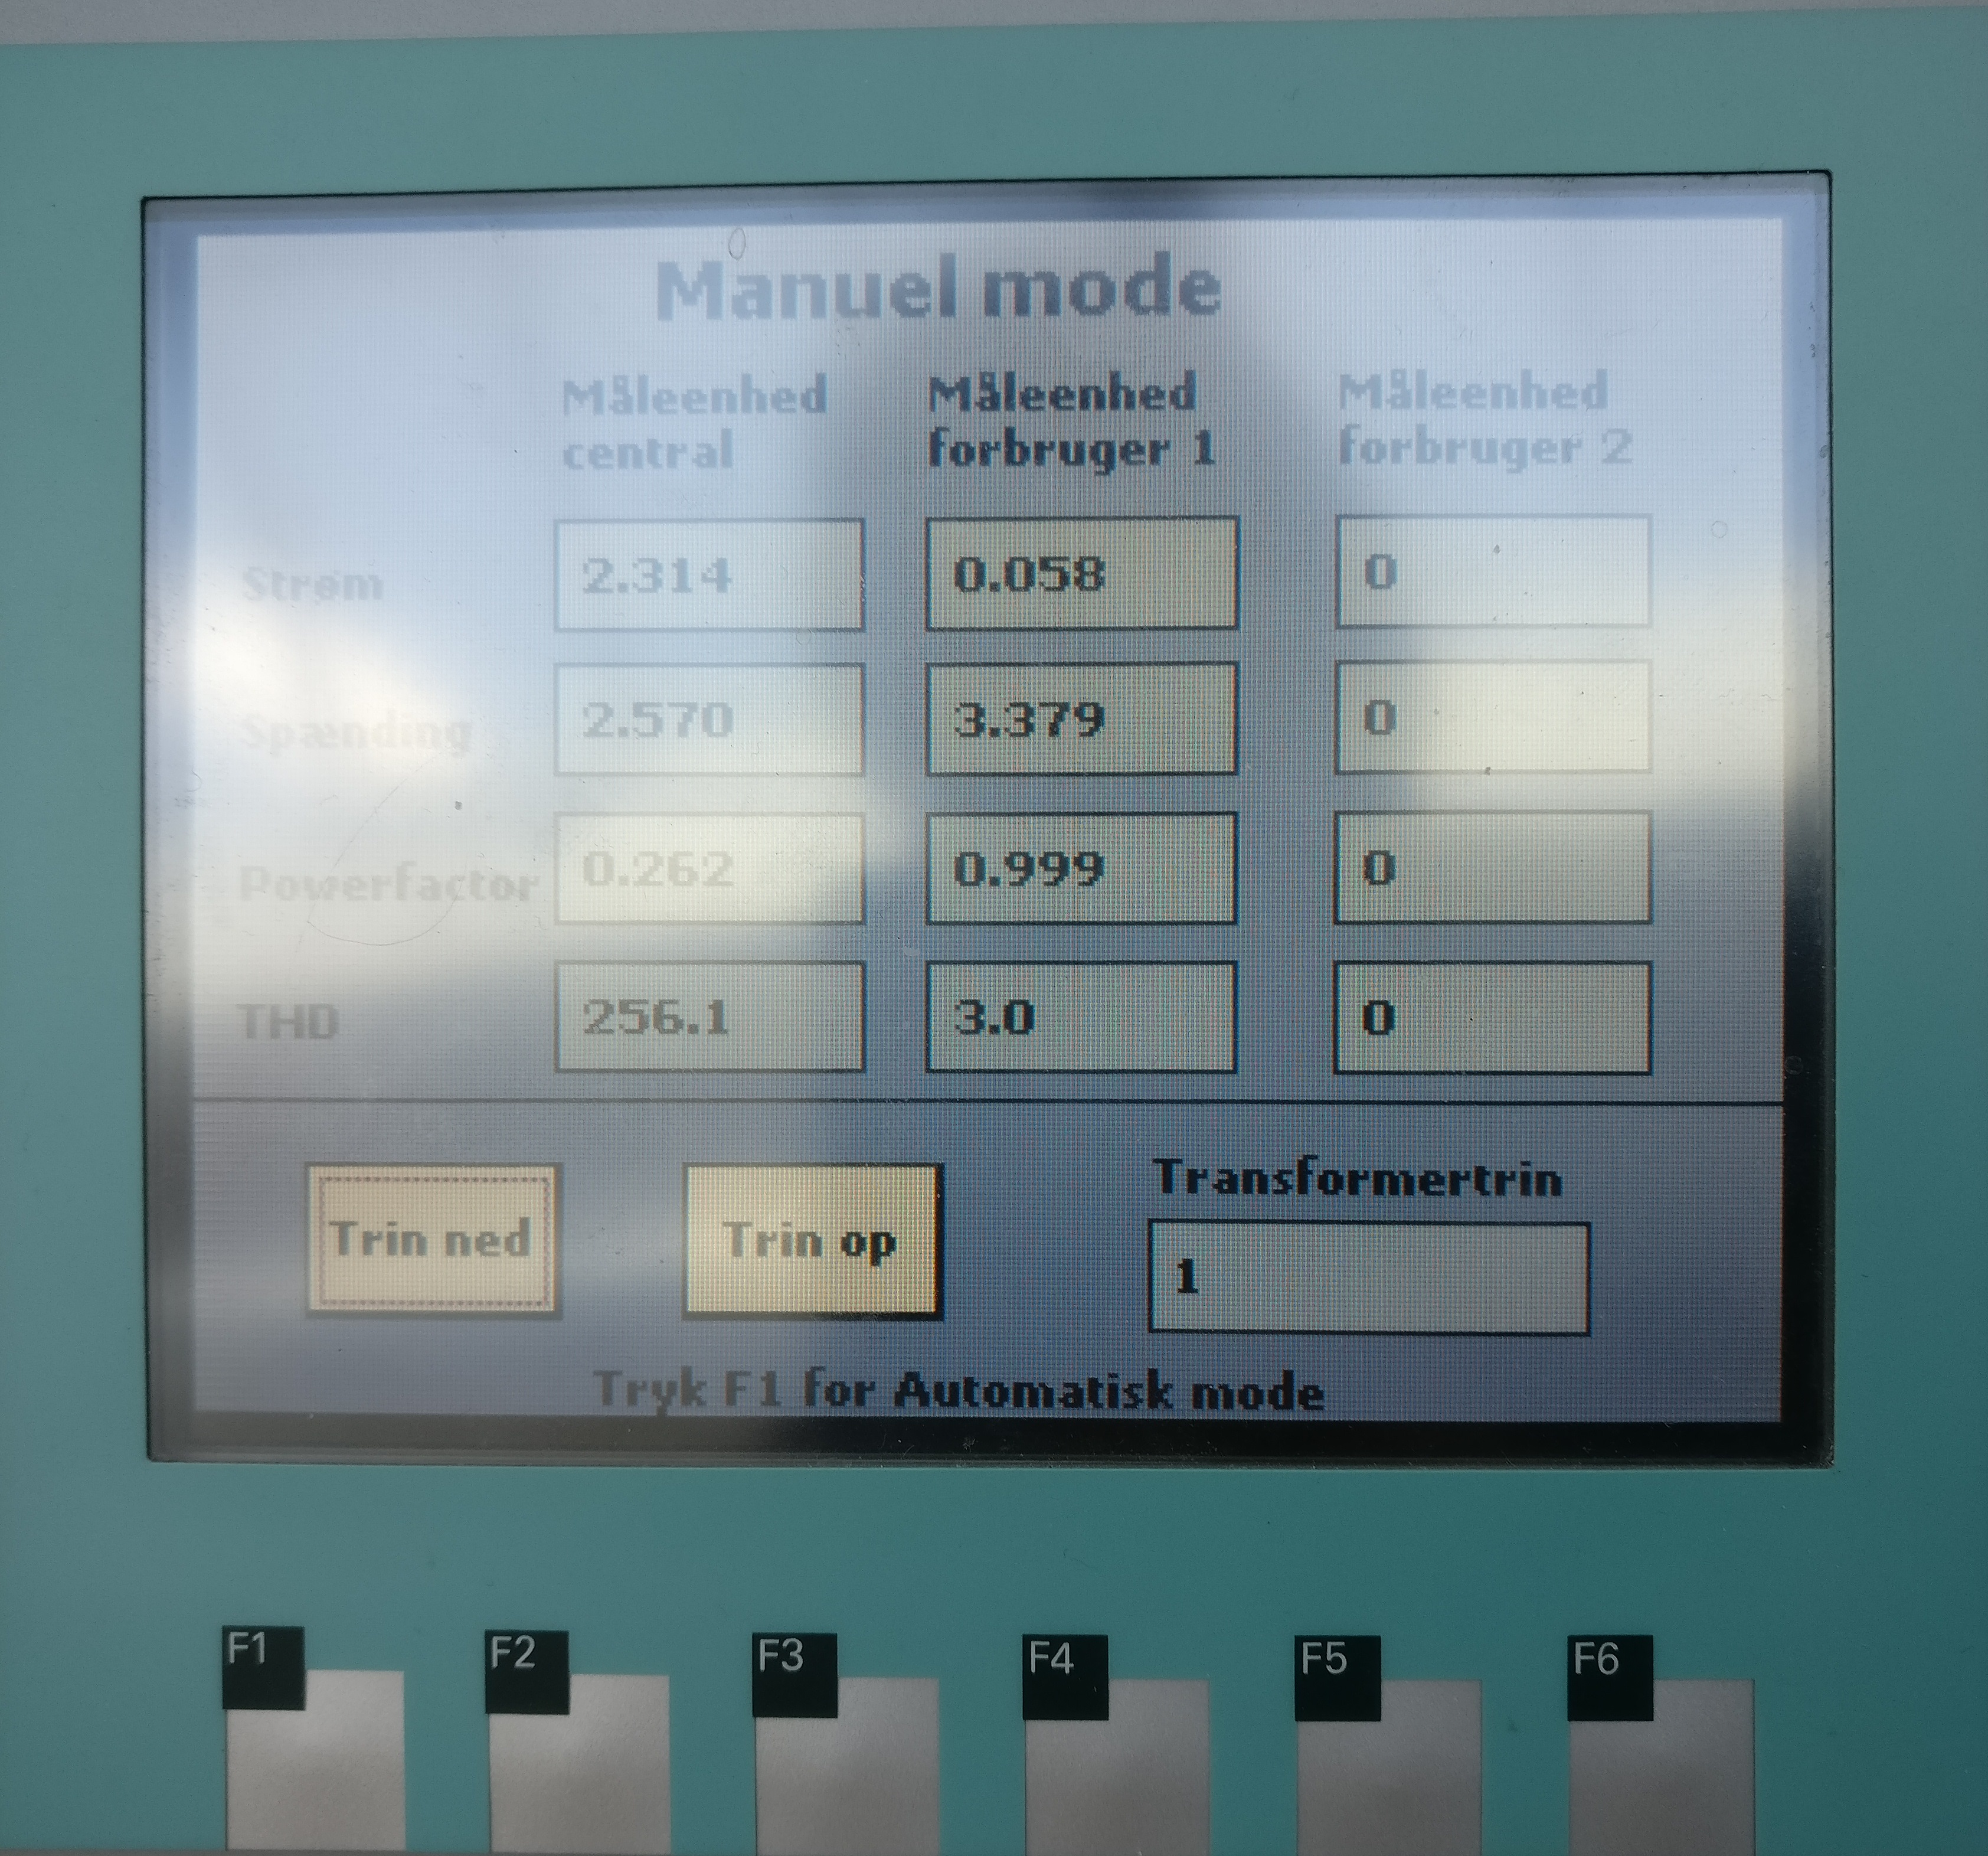
\includegraphics[width=0.7\textwidth]{Figure/INT4}
	\caption{Resultat af integrationstest 4, målteværdier.}
	\label{fig:INT4Mal}
\end{figure}



Opstillingen til den samlede integrationstest kan ses på figur \ref{fig:Opstilling1} og \ref{fig:Opstilling2}

\begin{figure}[H] 
	\centering
	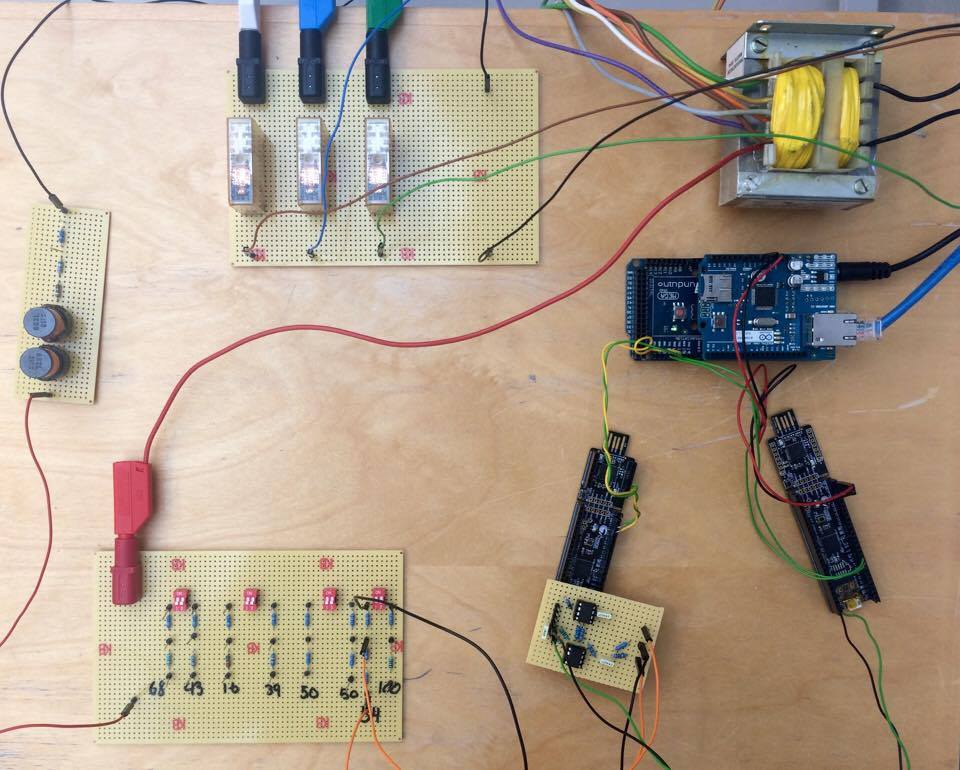
\includegraphics[width=0.7\textwidth]{Figure/Opstillingudenplc}
	\caption{Opstilling af samlet system uden PLC}
	\label{fig:Opstilling1}
\end{figure}

\begin{figure}[H] 
	\centering
	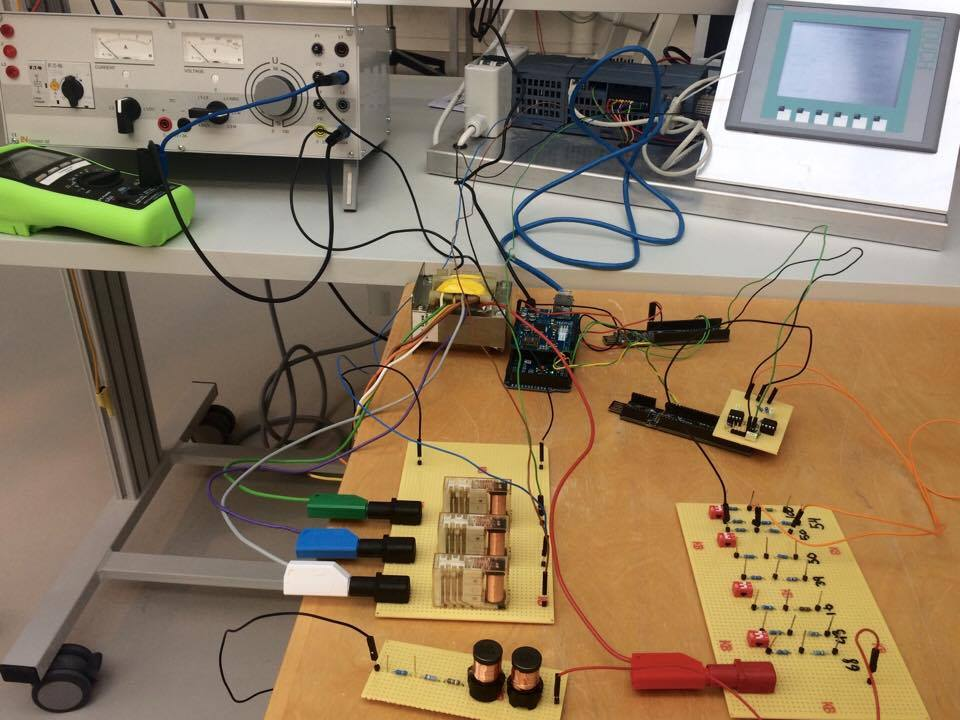
\includegraphics[width=0.7\textwidth]{Figure/Opstillingmedplc}
	\caption{Opstilling af samlet system med PLC}
	\label{fig:Opstilling2}
\end{figure}